\chapter{System Design and Architecture}
\label{Chapter-SystemDesign-Architecture}



\section{Overview diagram}
\begin{figure}[h!]
  \centering
  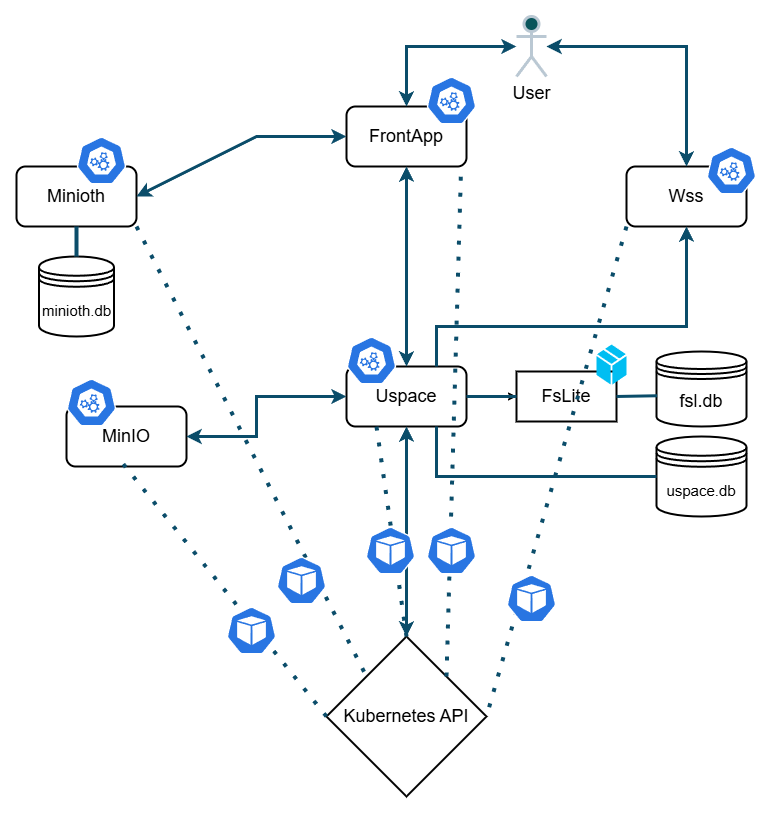
\includegraphics[width=1\textwidth]{Images/kuspace-overview.png}
  \caption{Kuspace System Overview}
  \label{fig:kuspace-overview}
\end{figure}


\begin{figure}[h!]
  \centering
  
\includegraphics[width=0.5\textwidth]{Images/kuspace-logo.png}
  \caption{Kuspace logo}
  \label{fig:kuspace-overview}
\end{figure}


\section{Minioth: Authentication Service}

Minioth~\cite{minioth} is a custom authentication and authorization microservice responsible for managing user identities and enforcing access control
within the system. It implements a secure token-based authentication model using JSON Web Tokens (JWT)~\cite{jwt-spec}, allowing users to authenticate
once and interact with other services securely.

\begin{figure}[h]
  \centering
  
\includegraphics[width=0.3\textwidth]{Images/minioth_logo_chatgpt_draft1.png}
  \caption{Minioth logo}
  \label{fig:miniothlogo}
\end{figure}

Minioth supports essential user and group management operations such as registration, login, group assignment, and permission checking.
It exposes a RESTful API~\cite{fielding-rest} that other services use to validate user tokens and retrieve identity-related metadata (e.g., UID, GID). 
This decouples authentication logic from the rest of the system, promoting modularity and reusability.

All user interactions begin with Minioth, and its integration is critical to enabling multi-user isolation, secure job execution, and 
controlled access to shared data resources.

Minioth aspires to become a fully capable identity provider!

\subsection{Authorization Details}

Minioth implements a simplified Role-Based Access Control (RBAC) model centered around user groups. Each user is assigned a unique primary group upon creation, which serves as the basis for resource ownership and sharing semantics. Group membership information is embedded in the issued JWTs, enabling downstream services to perform access checks without additional lookups.

At present, the system distinguishes between regular users and administrators. Membership in the \texttt{admin} group grants elevated privileges, including access to user and group management endpoints, system introspection, and key rotation. All other users are constrained to operations permitted within their assigned roles and groups.

\subsection{Authentication Details}

The Minioth authentication service implements secure, configurable user login and token issuance. Upon a successful login request via the \texttt{POST /login} endpoint, the system issues a JSON Web Token (JWT) containing the authenticated user's identity claims.

\paragraph{Token Signing Algorithm}
Clients can specify the desired signing algorithm by including the optional HTTP header:

\begin{quote}
\texttt{X-Auth-Signing-Alg: HS256} \quad or \quad \texttt{RS256}~\cite{jose-algorithms}
\end{quote}

\begin{itemize}
  \item \textbf{HS256} — HMAC using SHA-256~\cite{sha256-rfc6234}, with a system-defined shared secret.
  \item \textbf{RS256} — RSA signature using SHA-256, with a system-configured private/public key pair. 
  The public key is exposed via the JWKS endpoint (\texttt{/.well-known/jwks.json}).
\end{itemize}

If the header is omitted, the system uses the default signing algorithm defined in the configuration file. 
This design supports interoperability with external identity providers and ensures future extensibility toward OpenID Connect.

\paragraph{Password Hashing}
User passwords are never stored in plain text. Instead, all passwords are hashed using the \textbf{bcrypt}~\cite{bcrypt} 
algorithm prior to storage. The hashing cost (also referred to as the computational work factor) is system-defined and configurable. 
It controls the computational difficulty of the hashing process, allowing the system to be tuned for performance versus security:

\begin{algorithm}
\caption{Password Hashing using \texttt{bcrypt}}\label{alg:bcrypt}
\begin{algorithmic}[1]
\Procedure{HashPassword}{$password, cost$}
    \State $salt \gets \text{GenerateSalt}(cost)$
    \State $hash \gets \text{Bcrypt}(password, salt)$
    \State \Return $hash$
\EndProcedure
\end{algorithmic}
\end{algorithm}


A higher cost increases the time required to compute the hash, improving resistance to brute-force attacks at the expense of login speed.

\subsection{Pluggable Authentication Handlers}

Minioth is designed with extensibility in mind, offering a flexible backend architecture based on pluggable \textit{handlers}. A handler is a concrete implementation of a unified interface responsible for managing users, groups, and authentication state.

This architecture decouples the authentication logic from the underlying storage mechanism, enabling multiple interchangeable backends with minimal effort. All handlers implement the following interface:

\begin{algorithm}[H]
\caption{Abstract Handler Interface (pseudocode)}
\begin{algorithmic}
\Function{Init}{}
\EndFunction

\Function{UserAdd}{User}
  \State Returns: (UID, primaryGroup, Error)
\EndFunction

\Function{UserDel}{UID}
\EndFunction

\Function{UserMod}{User}
\EndFunction

\Function{UserPatch}{UID, Fields}
\EndFunction

\Function{GroupAdd}{Group}
  \State Returns: (GID, Error)
\EndFunction

\Function{GroupDel}{GID}
\EndFunction

\Function{GroupMod}{Group}
\EndFunction

\Function{GroupPatch}{GID, Fields}
\EndFunction

\Function{Authenticate}{Username, Password}
  \State Returns: User or Error
\EndFunction

\Function{Select}{ID}
  \State Returns: Any
\EndFunction

\Function{Purge}{}
\EndFunction

\Function{Close}{}
\EndFunction
\end{algorithmic}
\end{algorithm}



\paragraph{Available Handlers:}
\begin{itemize}
    \item \textbf{Database Handler:}  
    A fully featured implementation that uses a relational database backend (such as SQLite or DuckDB). This handler persists user, group, and credential data in structured tables, enabling query flexibility, indexing, and transactional safety.

    \item \textbf{Plain Handler:}  
    A minimalist implementation that stores user-related data in three flat files, following a UNIX-like structure:
    \begin{itemize}
        \item \texttt{mpasswd} — stores basic user account data (username, UID, GID)
        \item \texttt{mgroup} — stores group records (name, GID, members)
        \item \texttt{mshadow} — stores password hashes
    \end{itemize}
    This mode is particularly useful for lightweight deployments, testing, or portability.
\end{itemize}

Each handler supports core operations such as user/group creation, deletion, modification, and password-based authentication. 
By implementing the same interface, they are interchangeable at runtime, allowing the system to be easily configured for 
different deployment targets or performance/security trade-offs. 

New handlers suitable for other databases can be implemented.

\begin{figure}[h!]
  \centering
  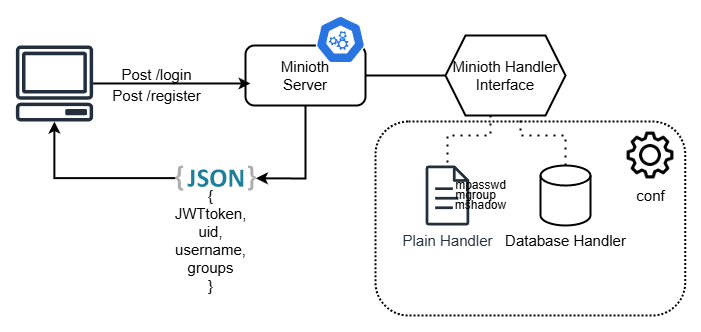
\includegraphics[width=1\textwidth]{Images/minioth-blockdiagram.png}
  \caption{Minioth Block Diagram}
  \label{fig:minioth-blockdiagram}
\end{figure}

\subsection{Minioth Public API Endpoints}

\begin{table}[H]
\centering
\resizebox{\textwidth}{!}{%
\begin{tabular}{|l|l|p{7cm}|c|}
\hline
\textbf{Method} & \textbf{Path} & \textbf{Description} & \textbf{Auth} \\
\hline
\hline
POST  & \texttt{/v1/register}            & Register a new user.                           & No  \\
POST  & \texttt{/v1/login}               & Authenticate and receive JWT token.            & No  \\
POST  & \texttt{/v1/passwd}              & Change password for the authenticated user.    & Yes (user/admin) \\
GET   & \texttt{/v1/user/me}             & Get information about the token's user.        & Token \\
GET   & \texttt{/v1/user/token}          & View current token details.                    & No \\
POST  & \texttt{/v1/user/refresh-token}  & Request a new access token using a refresh token. & No \\
GET   & \texttt{/v1/swagger/*any}        & Swagger UI for live API documentation.         & No \\
\hline
\hline
\end{tabular}%
}
\caption{Minioth public/user API endpoints}
\label{tab:minioth-public-endpoints}
\end{table}

\subsection{Minioth Admin API Endpoints}

\begin{table}[H]
\centering
\resizebox{\textwidth}{!}{%
\begin{tabular}{|l|l|p{7cm}|c|}
\hline
\textbf{Method} & \textbf{Path} & \textbf{Description} \\
\hline
\hline
GET    & \texttt{/v1/admin/audit/logs}      & Retrieve system audit logs. \\
POST   & \texttt{/v1/admin/hasher}          & Generate bcrypt hashes from plaintext passwords. \\
POST   & \texttt{/v1/admin/verify-password} & Compare a password against a stored hash. \\
GET    & \texttt{/v1/admin/users}           & List all registered users. \\
GET    & \texttt{/v1/admin/groups}          & List all groups and their members. \\
POST   & \texttt{/v1/admin/useradd}         & Add a new user to the system. \\
DELETE & \texttt{/v1/admin/userdel}         & Delete a user by UID or username. \\
PATCH  & \texttt{/v1/admin/userpatch}       & Update selected fields of a user. \\
PUT    & \texttt{/v1/admin/usermod}         & Fully replace a user record. \\
POST   & \texttt{/v1/admin/groupadd}        & Create a new group. \\
PATCH  & \texttt{/v1/admin/grouppatch}      & Update specific fields of a group. \\
PUT    & \texttt{/v1/admin/groupmod}        & Fully update a group definition. \\
DELETE & \texttt{/v1/admin/groupdel}        & Remove a group from the system. \\
POST   & \texttt{/v1/admin/rotate}          & Rotate the JWT signing key in use. \\
GET    & \texttt{/v1/admin/system-conf}     & View current server configuration. \\
\hline
\hline
\end{tabular}%
}
\caption{Minioth public/admin API endpoints}
\label{tab:minioth-public-endpoints}
\end{table}

Essentially admin features include full user/group lifecycle management and 
audit logging, key rotation and token inspection mechanisms.

An Authorization header is required with the JWT token as a Bearer.

\subsection{Integration}

Minioth is integrated into the overall system architecture as a Kubernetes StatefulSet, with user and group data persisted on a dedicated Persistent Volume Claim (PVC). It serves as the central authentication authority by issuing JWT tokens consumed by other services, primarily the Frontend application, to authorize user actions.

To ensure secure inter-service communication, all microservices, including Minioth, share a common \texttt{ServiceSecret} key. This key enables mutual trust and token verification across services. Additionally, the JWT signing key is generated at deployment time via a configurable secret generator and securely injected into the Minioth service configuration.


\newpage



\section{Uspace: Central Orchestration and Job Management Service}
\label{sec:uspace}

The \textbf{Uspace} service constitutes the core of the system’s architecture, 
acting as the central orchestration unit that coordinates job scheduling, 
storage access, and user-level interaction with analytical resources. 
It is built with extensibility and modularity in mind, offering a consistent 
interface between users, applications, and the underlying infrastructure.

\subsection{Responsibilities and Purpose}

Uspace maintains the persistent state of the system through:
\begin{itemize}
    \item A resource and volume metadata store powered by the \texttt{FsLite} module.
    \item A local database (SQLite or DuckDB) for tracking user-submitted jobs and available applications.
    \item A job scheduling and dispatch pipeline which integrates with the Kubernetes API.
\end{itemize}

Uspace exposes a RESTful API to authenticated users and administrators, supporting operations such as uploading datasets, browsing resources, and launching computational jobs.

\newpage

\begin{table}[H]
\centering
\resizebox{\textwidth}{!}{%
\begin{tabular}{|l|l|p{9cm}|c|}
\hline
\textbf{Method} & \textbf{Path} & \textbf{Description} & \textbf{Requires \texttt{Access-Target}} \\
\hline
GET & \texttt{/healthz} & Health check endpoint. & No \\
GET/POST & \texttt{/api/v1/job} & Submit or list jobs. & No \\
GET/POST & \texttt{/api/v1/app} & List available tools (applications). & No \\
GET & \texttt{/api/v1/resources} & List resources (“ls” equivalent). & Yes \\
POST & \texttt{/api/v1/resource/upload} & Upload a new resource file. & Yes \\
GET & \texttt{/api/v1/resource/preview} & Preview a resource. & Yes (Read) \\
GET & \texttt{/api/v1/resource/download} & Download a resource. & Yes (Read) \\
DELETE & \texttt{/api/v1/resource/rm} & Delete a resource. & Yes (Write) \\
POST & \texttt{/api/v1/resource/cp} & Copy a resource. & Yes (Read) \\
PATCH & \texttt{/api/v1/resource/mv} & Move/rename a resource. & Yes (Write) \\
PATCH & \texttt{/api/v1/resource/permissions} & Change resource permissions. & Yes (Owner) \\
PATCH & \texttt{/api/v1/resource/ownership} & Change resource ownership. & Yes (Owner) \\
PATCH & \texttt{/api/v1/resource/group} & Change associated group. & Yes (Owner) \\
\hline
\end{tabular}
}
\caption{Uspace User API Endpoints}
\label{tab:uspace-user-endpoints}
\end{table}


\begin{table}[H]
\centering
\resizebox{\textwidth}{!}{%
\begin{tabular}{|l|l|p{9cm}|}
\hline
\textbf{Method} & \textbf{Path} & \textbf{Description} \\
\hline
GET/POST/PUT/DELETE/PATCH & \texttt{/api/v1/admin/volumes} & Full volume management API. \\
DELETE/PUT & \texttt{/api/v1/admin/job} & Administrative job control (e.g., delete jobs). \\
GET/POST/PATCH/DELETE & \texttt{/api/v1/admin/user/volume} & Manage user-volume mappings. \\
GET/POST/PUT/DELETE & \texttt{/api/v1/admin/app} & Manage available applications/tools. \\
GET & \texttt{/api/v1/admin/system-conf} & View current system configuration. \\
GET & \texttt{/api/v1/admin/system-metrics} & System metrics via Kubernetes API. \\
\hline
\end{tabular}
}
\caption{Uspace Admin API Endpoints}
\label{tab:uspace-admin-endpoints}
\end{table}

\subsection{Middleware and Access Control}

The Uspace API applies layered middleware to enforce authentication, authorization, and request context binding.

In particular, API endpoints require a custom HTTP header named \texttt{Access-Target}, which encodes the target resource and the user identity. The header follows this format:

\begin{verbatim}
Access-Target: <volume_id>:<volume_name>:<resource_path> 
<user_id>:[group_id1,group_id2,...]
\end{verbatim}

The middleware parses this value to construct an \texttt{AccessClaim} object, which is then used to evaluate permissions through FsLite. This mechanism abstracts identity and access metadata away from individual endpoint logic and enforces consistency across resource operations.

Only authorized users (based on ownership or group permissions) can perform operations such as previewing, downloading, modifying, or deleting resources.

Furthermore, all API groups apply the \texttt{serviceAuth} middleware for validating a ServiceSecret common in the Service and verifying the caller is only a service in the system.

\subsection{Core Structure}

At the heart of the system lies the \texttt{UService} object, which encapsulates the configuration, runtime engine, and modular components responsible for storage, job handling, and resource management. Its composition is summarized as follows:

\begin{itemize}
    \item \textbf{Configuration (\texttt{config})}: Encapsulates all environment-based settings loaded during service initialization. This allows flexible configuration for both development and production deployments.
    
    \item \textbf{Web Engine (\texttt{Engine})}: A Gin-based HTTP server that handles incoming API requests and routes them to appropriate handlers. It also includes middleware for authentication and authorization.
    
    \item \textbf{Storage Backend (\texttt{storage})}: Implements the \texttt{StorageSystem} interface. In this system, it uses a MinIO-based implementation for interacting with S3-compatible object storage. The interface, however, allows for future pluggability (e.g., plain file volumes).
    
    \item \textbf{Job Database Handler (\texttt{jdbh})}: Provides access to the local DuckDB or SQLite database used to track job submissions, statuses, and registered analytical applications.
    
    \item \textbf{Filesystem Metadata Layer (\texttt{fsl})}: An instance of FsLite, used as an internal metadata engine for enforcing user-based access controls and tracking virtual filesystem hierarchies over the object store.
    
    \item \textbf{Job Dispatcher (\texttt{jdp})}: Orchestrates the submission and lifecycle of analytical jobs. It abstracts the underlying execution backend (e.g., Kubernetes or Docker), enabling future extensibility via the \texttt{JobDispatcher} interface.
\end{itemize}


\newpage

\subsection{Storage Provider Abstraction}

The \texttt{StorageSystem} interface defines the contract for interacting with storage backends. Below is a description of its main methods:

\begin{algorithm}[H]
\caption{Abstract \texttt{StorageSystem} Interface (pseudocode)}
\begin{algorithmic}[1]

\Function{DefaultVolume}{local: Bool}
  \State \Return default volume identifier as String
\EndFunction

\Function{CreateVolume}{volume: Any}
  \State \Return Error if creation fails
\EndFunction

\Function{SelectVolumes}{criteria: Map[String, Any]}
  \State \Return matching volumes or Error
\EndFunction

\Function{SelectObjects}{criteria: Map[String, Any]}
  \State \Return matching objects or Error
\EndFunction

\Function{Insert}{object: Any}
  \State \Return CancelFunc, Error
\EndFunction

\Function{Download}{object: Any}
  \State \Return CancelFunc, Error
\EndFunction

\Function{Stat}{object: Any}
  \State \Return metadata or Error
\EndFunction

\Function{Remove}{object: Any}
  \State \Return Error
\EndFunction

\Function{RemoveVolume}{volume: Any}
  \State \Return Error
\EndFunction

\Function{Update}{metadata: Map[String, String]}
  \State \Return Error
\EndFunction

\Function{Copy}{source: Any, dest: Any}
  \State \Return Error
\EndFunction

\Function{Share}{method: String, object: Any}
  \State \Return SharingDescriptor or Error
\EndFunction

\end{algorithmic}
\end{algorithm}


\newpage
\subsection{Storage Control}
Uspace as mentioned handles storage in two layers. 
\begin{itemize}

\item  The metadata layer that includes access control is consisted of \texttt{FsLite} module which also 
enforces authorization on the resources.
\item The \texttt{StorageSystem} for physical storage, MinIO, and its API is accessed by a custom Go MinIO client.
\end{itemize}


\begin{figure}[h]
  \centering
  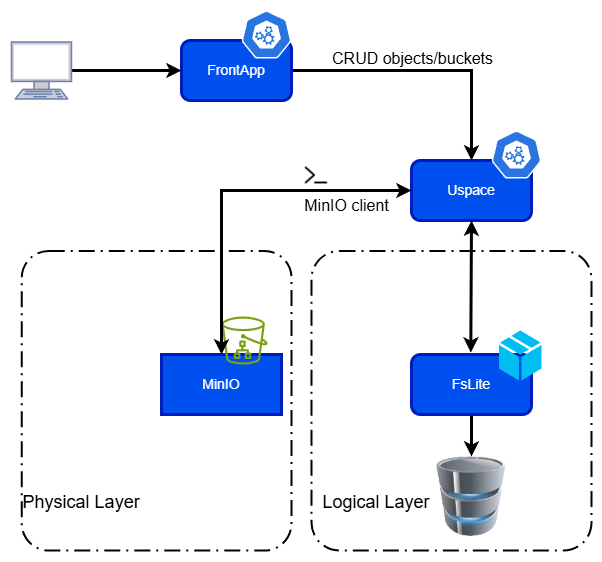
\includegraphics[width=1\textwidth]{Images/UspaceBlockDiagram.drawio.png}
  \caption{Uspace Storage Overview}
  \label{fig:uspace-storage-overview}
\end{figure}

\subsection{Job Dispatcher and Executor}

Uspace includes a pluggable job dispatching mechanism defined by the \texttt{JobDispatcher} interface,
as well as a job execution mechanism defined by the \texttt{JobExecutor} interface:

\begin{algorithm}[H]
\caption{Abstract \texttt{JobDispatcher} Interface (pseudocode)}
\label{alg:job-dispatcher}
\begin{algorithmic}[1]

\Function{Start}{}
  \State Initialize and begin dispatching system
\EndFunction

\Function{PublishJob}{job: Job}
  \State Submit a single job for dispatch
  \State \Return Error on failure
\EndFunction

\Function{PublishJobs}{jobs: List[Job]}
  \State Submit a batch of jobs
  \State \Return Error on failure
\EndFunction

\Function{RemoveJob}{jobID: Integer}
  \State Cancel or remove job with given ID
  \State \Return Error on failure
\EndFunction

\Function{RemoveJobs}{jobIDs: List[Integer]}
  \State Remove multiple jobs
  \State \Return Error on failure
\EndFunction

\Function{Subscribe}{job: Job}
  \State Register job for event handling or feedback
  \State \Return Error on failure
\EndFunction

\end{algorithmic}
\end{algorithm}

\begin{algorithm}[H]
\caption{Abstract \texttt{JobExecutor} Interface (pseudocode)}
\begin{algorithmic}
\Function{ExecuteJob}{job}
  \State Returns: Error
\EndFunction

\Function{CancelJob}{job}
  \State Returns: Error
\EndFunction

\end{algorithmic}
\end{algorithm}



The default implementation is a \texttt{JobManager}, which maintains queues and internal execution tracking. It uses a \texttt{JobExecutor} to actually launch jobs using one of two backends:
\begin{itemize}
    \item \textbf{DockerExecutor}: Launches jobs in local Docker containers for testing.
    \item \textbf{KubernetesExecutor}: Launches Kubernetes Jobs via the API for production workloads.
\end{itemize}

This separation of concerns enables the system to evolve with future support for alternative execution engines such as serverless functions or distributed clusters.

\textbf{Job Specification}: Each submitted job is described by a structured payload that defines its resource requirements, execution logic, and metadata.

The job object includes:

\begin{itemize}
    \item \textbf{Identifiers:} \texttt{JID} (Job ID), \texttt{UID} (User ID).
    \item \textbf{Resource Requirements:} CPU, memory, and ephemeral storage requests/limits.
    \item \textbf{Execution Parameters:} \texttt{Parallelism}, \texttt{Timeout}, \texttt{Priority}.
    \item \textbf{Paths:} \texttt{Input} and \texttt{Output} resource references.
    \item \textbf{Logic:} A predefined \texttt{Logic} (e.g., ``duckdb'') and a \texttt{LogicBody} representing the code or command to be executed.
    \item \textbf{Environment:} An optional key-value map of environment variables.
    \item \textbf{Status Tracking:} Includes current \texttt{Status}, \texttt{CreatedAt}, \texttt{CompletedAt}, and a boolean \texttt{Completed} flag.
\end{itemize}

Jobs are submitted through the Uspace API, validated, and dispatched for execution by the internal job manager. The structure supports extensibility for both containerized tools and script execution across different runtimes.

\subsection{Job Execution Pipeline}
\textbf{Job Execution} in Uspace follows as:
\begin{enumerate}
  \item The user submits a job definition via \texttt{/job}.
  \item The \texttt{JobDispatcher} validates and prepares the job.
  \item The \texttt{JobManager} handles scheduling and preparation for Kubernetes.
  \item The \texttt{JobExecutor} decides upon the existing imaged applications, and sets up the appropriate variables and connections for I/O to the Storage System
  \item The \texttt{JobExecutor} then launches the containerized workload on the Engine Execution Model (e.g Kubernetes API Jobs).
  \item Runtime results are streamed to WSS and the output is saved on the Storage Provider (MinIO) of the path specified.
\end{enumerate}

All jobs are tracked in the local job database with associated metadata, status, timestamps, and references to input/output files.

\subsection{Job Scheduling}

The \texttt{Uspace} service includes an embedded job scheduling mechanism implemented by the \texttt{JobManager} component. It operates on a producer-consumer model, where jobs submitted by authenticated users are pushed into a bounded queue (\texttt{jobQueue}). The size of this queue is configurable via \texttt{UspaceJobQueueSize}, defaulting to 100 entries.

Job execution is handled concurrently by a worker pool, constrained by a configurable parameter (\texttt{UspaceJobMaxWorkers}). Each job is processed in a dedicated goroutine, with the pool enforced via a buffered channel (\texttt{workerPool}) to prevent system overload.

When a job is dequeued, it is dispatched to the selected \texttt{JobExecutor}—either Docker-based or Kubernetes-based—determined during service initialization. This separation allows for modular testing and cloud-native deployment.

If the job queue is full, submissions are rejected, providing backpressure to upstream services or users. This model ensures that the system maintains a predictable load and resource profile.

\newpage

\begin{figure}[h]
  \centering
  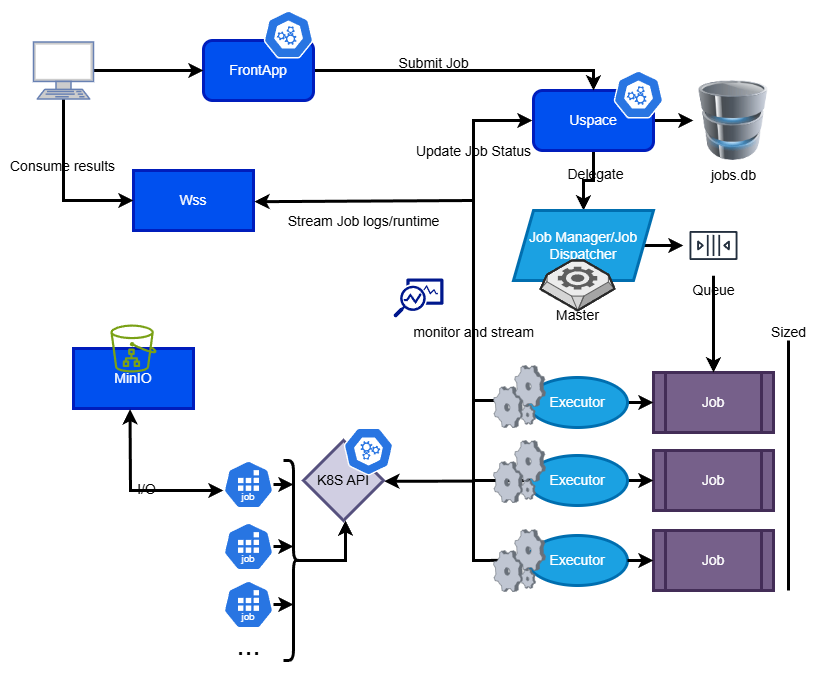
\includegraphics[width=1\textwidth]{Images/job-lifecycle.png}
  \caption{Job Lifecycle}
  \label{fig:job-lifecycle}
\end{figure}


\subsection{Available Applications}

The Uspace system supports a set of containerized applications that can be executed as jobs. These applications are defined as Docker images with a uniform execution contract. Each application:

\begin{itemize}
    \item Receives the input and output paths via environment variables.
    \item Uses preconfigured MinIO credentials to fetch and store data.
    \item Executes its logic using the input file(s) and writes the results to the specified output location in MinIO.
\end{itemize}

The current applications integrated into the system are shown in Table~\ref{tab:uspace-apps}. Each is versioned and can be expanded or modified independently.

\begin{table}[H]
\centering
\resizebox{\textwidth}{!}{%
\begin{tabular}{|l|l|l|l|l|l|}
\hline
\textbf{Name} & \textbf{Image} & \textbf{Description} & \textbf{Version} & \textbf{Author} & \textbf{Status} \\
\hline
duckdb & \texttt{kuspace:applications-duckdb-v1} & DuckDB SQL on MinIO object I/O & v1 & k & available \\
pypandas & \texttt{kuspace:applications-pypandas-v1} & Python Pandas on MinIO object I/O & v1 & k & available \\
octave & \texttt{kuspace:applications-octave-v1} & Octave code with MinIO object I/O & v1 & k & available \\
ffmpeg~\cite{ffmpeg} & \texttt{kuspace:applications-ffmpeg-v1} & FFmpeg commands on MinIO object I/O & v1 & k & available \\
caengine~\cite{caengine-thesis} & \texttt{kuspace:applications-caengine-v1} & Custom engine with MinIO object I/O & v1 & k & available \\
bash & \texttt{kuspace/applications-bash-v1} & Run Bash commands on objects & v1 & k & available \\
\hline
\end{tabular}
}
\caption{Currently supported applications in Uspace}
\label{tab:uspace-apps}
\end{table}


\begin{figure}[h!]
  \centering
  \begin{subfigure}[b]{0.1\textwidth}
    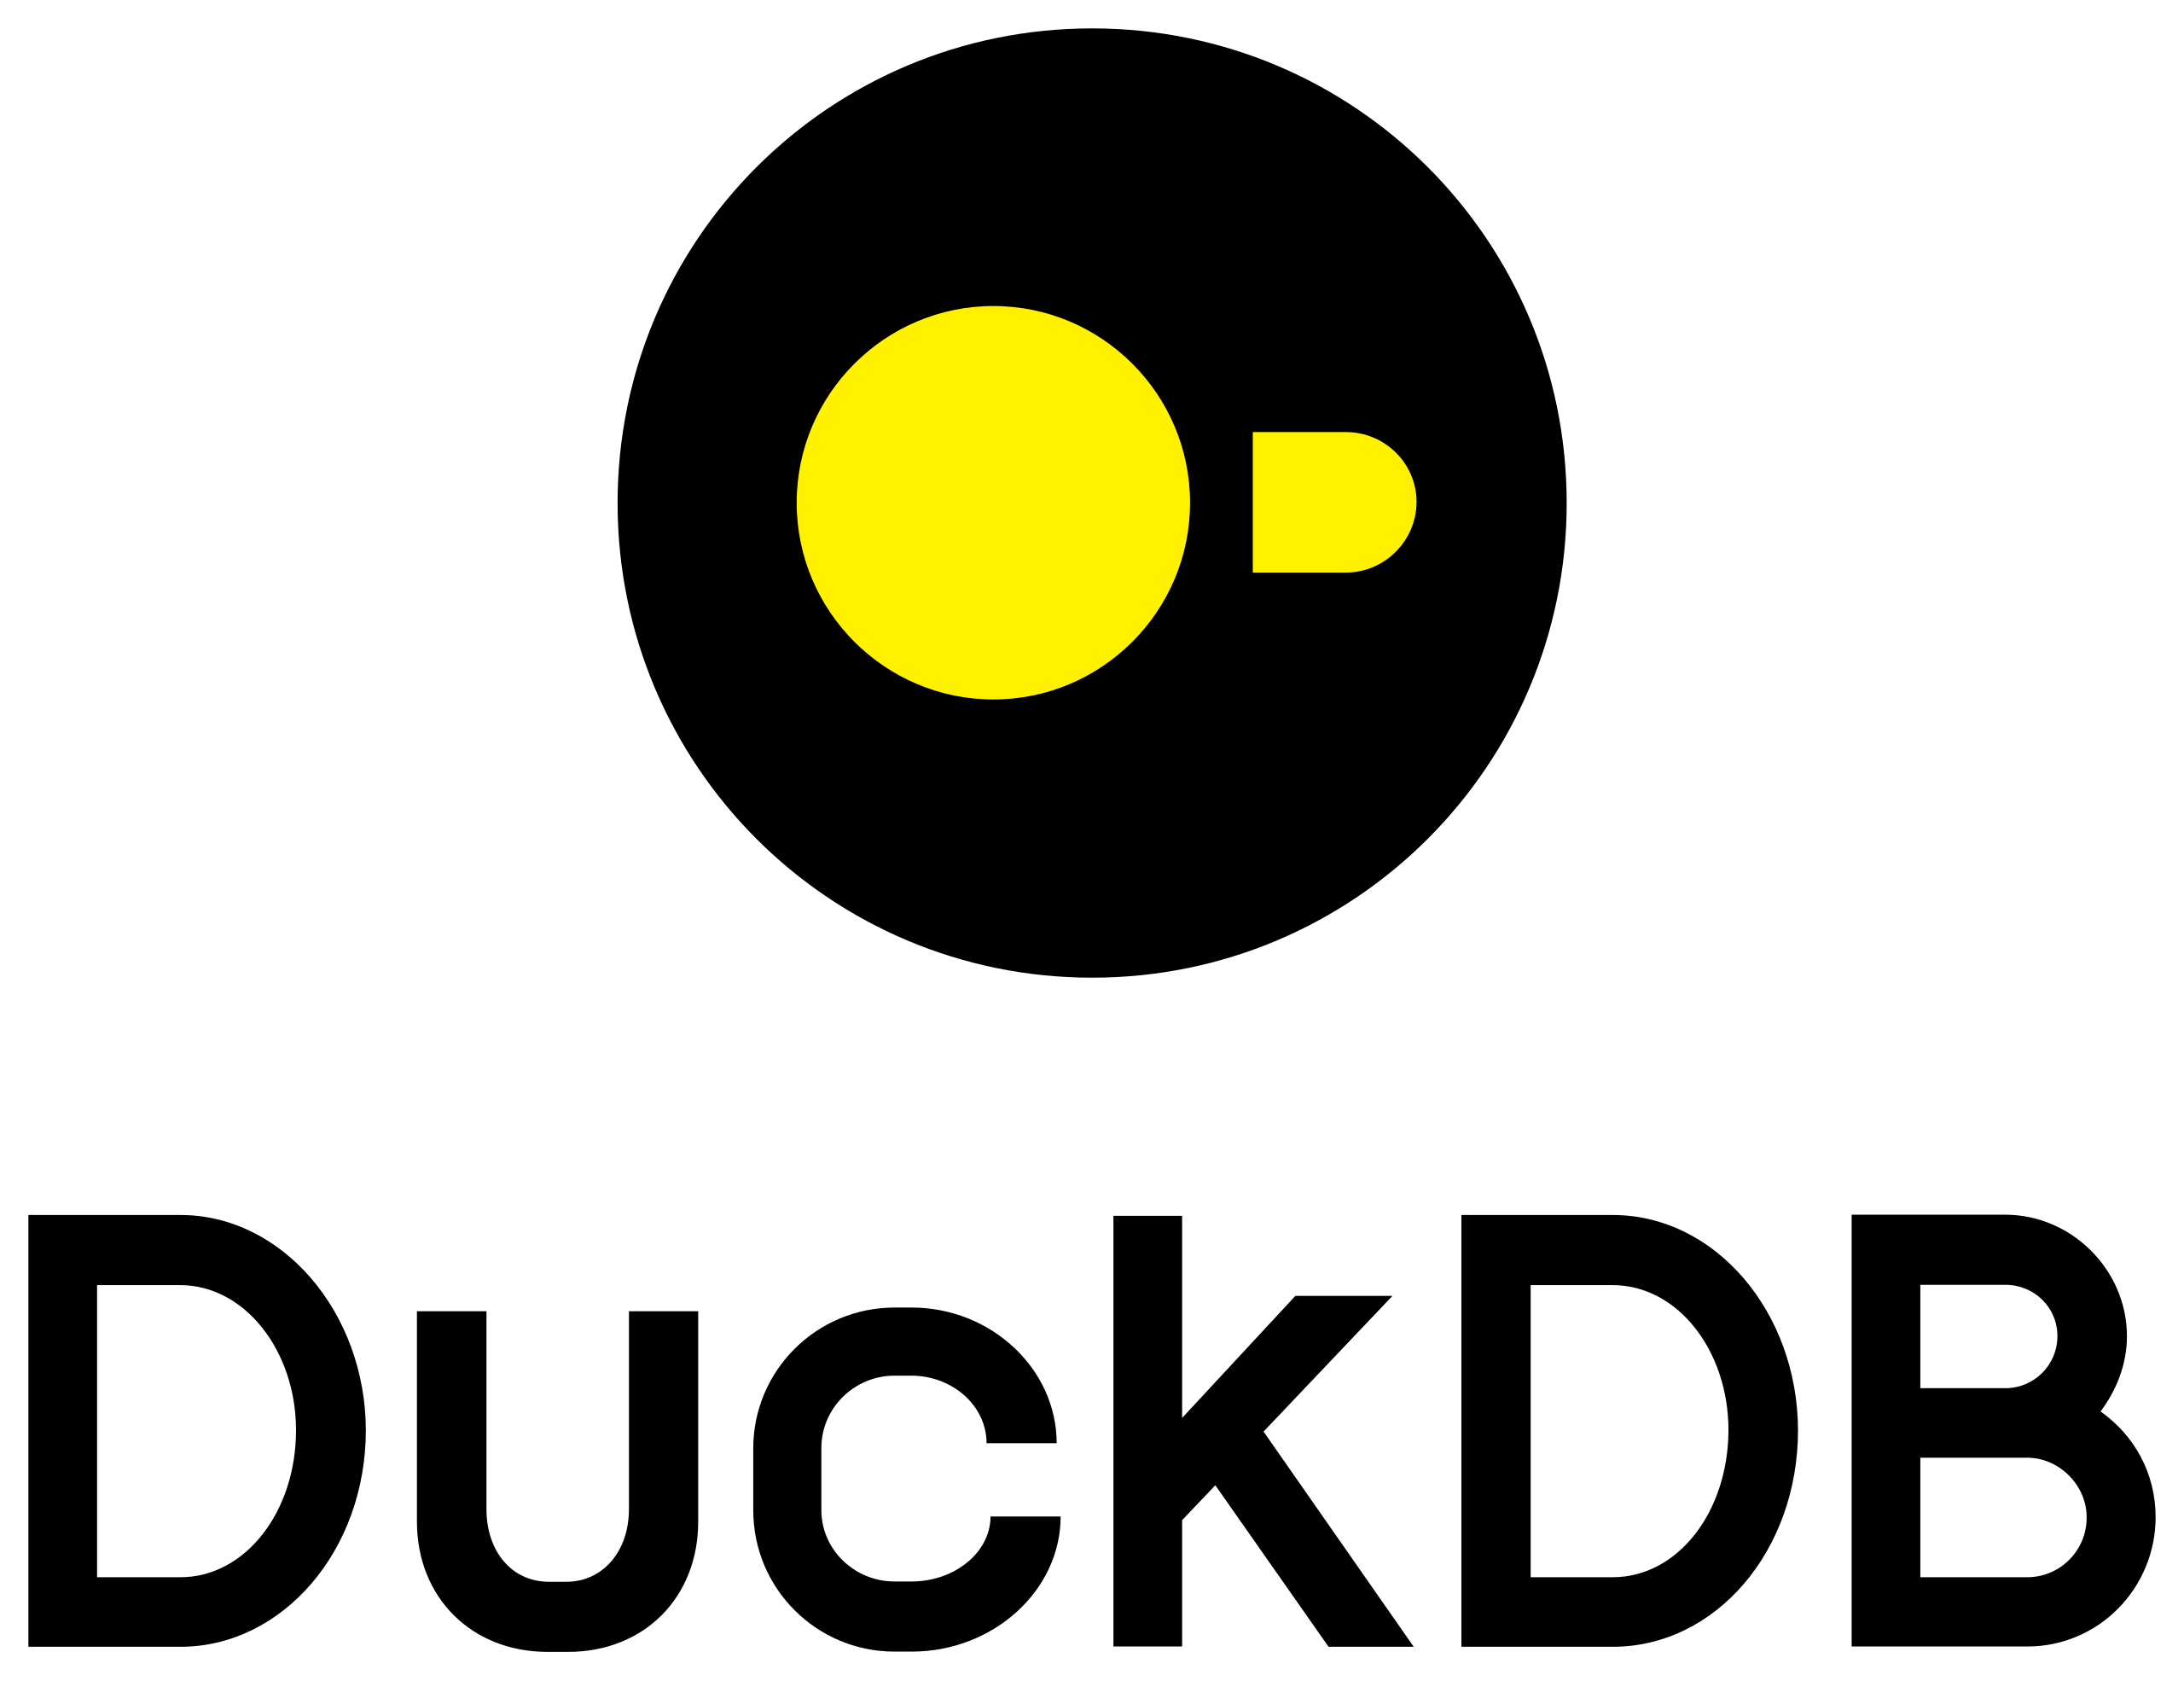
\includegraphics[width=\textwidth]{Images/DuckDB_logo.svg.png}
    \label{fig:duckdb}
  \end{subfigure}
  \hfill
  \begin{subfigure}[b]{0.1\textwidth}
    
\includegraphics[width=\textwidth]{Images/octave.png}
    \label{fig:octave}
  \end{subfigure}
  \hfill
  \begin{subfigure}[b]{0.1\textwidth}
    
\includegraphics[width=\textwidth]{Images/Pandas_logo.svg.png}
    \label{fig:pandas}
  \end{subfigure}

  \par\vspace{1em} % New row with vertical space

  \begin{subfigure}[b]{0.1\textwidth}
    
\includegraphics[width=\textwidth]{Images/ffmpeg.png}
    \label{fig:ffmpeg}
  \end{subfigure}
  \hfill
  \begin{subfigure}[b]{0.1\textwidth}
    
\includegraphics[width=\textwidth]{Images/bash.png}
    \label{fig:bash}
  \end{subfigure}
  \hfill
  \begin{subfigure}[b]{0.1\textwidth}
    
\includegraphics[width=\textwidth]{Images/default_logo.png}
    \label{fig:caengine}
  \end{subfigure}

  \caption{Available Kuspace Applications}
  \label{fig:authservices}
\end{figure}


\subsection{Integration and Security}

Uspace authenticates user actions via JWT tokens issued by the Minioth authentication service. It verifies group memberships and resource permissions using the FsLite metadata store and enforces a Unix-style access control model.

The service is deployed as a Kubernetes \texttt{StatefulSet}, ensuring persistent identity and stable storage across restarts. Uspace stores its embedded database and FsLite metadata in a \texttt{PersistentVolumeClaim} (PVC), ensuring durability of user and job metadata.

Administrators can assign storage volumes, manage user data, inspect system metrics, and access operational logs through authenticated admin endpoints. All internal microservice communications are secured using a shared \texttt{ServiceSecret}, available at runtime to authorized components only.




\newpage



\section{Fslite}

\begin{figure}[h]
  \centering
  
\includegraphics[width=0.3\textwidth]{Images/fslite_chatgpt_draft1.png}
  \caption{FsLite logo}
  \label{fig:fslogo}
\end{figure}


FsLite is a modular metadata and volume management system that can operate either as an embedded library or as a standalone microservice. It is used within the Uspace module to abstract and manage virtual storage concepts, such as user volumes, datasets, and permissions, before interacting with the physical storage backend (MinIO).

\begin{figure}[h!]
  \centering
  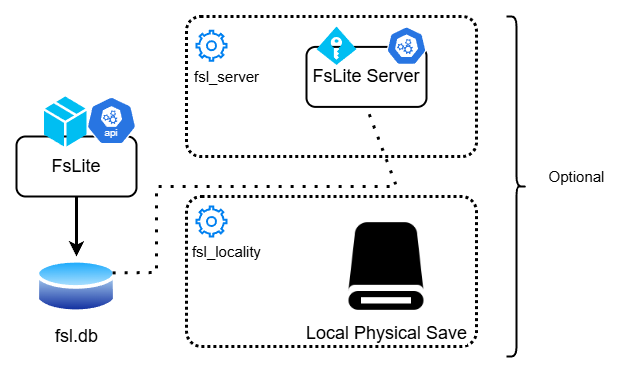
\includegraphics[width=1\textwidth]{Images/fsl.png}
  \caption{FsLite Block Diagram}
  \label{fig:fslite-blockdiagram}
\end{figure}

\subsection{Purpose and Design}

The key design goal of FsLite is to provide a lightweight, configurable system to handle logical resource management, including tracking objects, managing access control, and storing volume definitions. It uses an embedded relational database (SQLite or DuckDB, depending on configuration) for metadata persistence.

FsLite enables the system to:
\begin{itemize}
    \item Create and track logical volumes and resource entries before physical allocation.
    \item Maintain metadata about files, directories, and symbolic links.
    \item Perform access control enforcement based on user and group ownership.
    \item Act as an intermediate layer before delegating large-scale I/O to MinIO.
\end{itemize}

\subsection{Deployment and Initialization}

When deployed in standalone mode, FsLite operates as a RESTful microservice using the Gin web framework. It initializes by connecting to the configured database and optionally preparing a physical volume path on the local filesystem. If enabled, it creates a default volume using the directory and capacity limits specified in the system configuration.

The admin credentials (access and secret key) are inserted during startup. Optionally, the system can bypass authentication for development or local deployments.

\subsection{API Endpoints}

FsLite exposes a structured API grouped under a versioned path. The endpoints are divided into authentication, volume management, and resource operations. Key endpoints include:

\begin{table}[H]
\centering
\resizebox{\textwidth}{!}{%
\begin{tabular}{|l|l|p{9cm}|}
\hline
\textbf{Method} & \textbf{Path} & \textbf{Description}\\
\hline
\hline
POST              & \texttt{/login}                     & Authenticate and receive a token.\\
POST              & \texttt{/admin/register}            & Authenticate and receive JWT token.\\
POST              & \texttt{/admin/volume/new}          & Change password for the authenticated user.\\
DELETE            & \texttt{/admin/volume/delete}       & Delete a specified volume\\
GET               & \texttt{/admin/volume/get}          & Retrieve information about a logical volume\\
GET               & \texttt{/admin/resource/get}        & Retrieve metadata of multiple resources \\ 
GET               & \texttt{/admin/resource/stat}       & Retrieve more detailed metadata of a specific resource.\\
DELETE            & \texttt{/admin/resource/delete}     & Delete a specified resource.\\
POST              & \texttt{/admin/resource/upload}     & Upload resource content to volume.\\
GET               & \texttt{/admin/resource/download}   & Download a resource from storage.\\
GET/PATCH/DELETE  & \texttt{/admin/user/voumes}         & CRUD user volumes.\\
\hline
\hline
\end{tabular}%
}
\caption{FsLite public API endpoints}
\label{tab:fslite-public-endpoints}
\end{table}

\subsection{Integration in the System}

FsLite is integrated into the Uspace module, which delegates resource and volume tracking tasks to it. This modular separation allows Uspace to offload concerns related to volume capacity, ownership verification, and metadata persistence to FsLite.

Its database-backed design allows stateless operation from the perspective of the consuming services. It also enables simulation of filesystem-like permissions using UNIX-style ownership and mode bits.

\subsubsection{Local vs Remote Operation}

FsLite can operate in two modes:
\begin{itemize}
    \item \textbf{Local Mode:} FsLite creates a data directory on the host machine and directly stores uploaded files, suitable for testing or single-node deployments.
    \item \textbf{Remote Mode:} FsLite acts purely as a metadata layer; files are stored in MinIO or other backends using volume references.
\end{itemize}

\begin{figure}[h!]
  \centering
  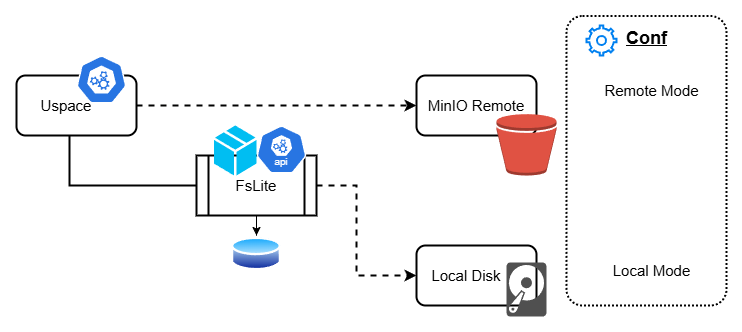
\includegraphics[width=1\textwidth]{Images/fslite-block-diagram.png}
  \caption{FsLite Integration}
  \label{fig:fslite-integration}
\end{figure}



\section{Storage Layer (MinIO)}

MinIO serves as the system's object storage backend, offering a scalable, S3-compatible API for storing and retrieving binary data such as 
uploaded datasets and job output files. It is tightly integrated with Kubernetes and can be accessed from within containers via network mounts 
or HTTP APIs.

Each user’s data is stored under isolated bucket structures or path prefixes, ensuring access control through both object path naming 
conventions and Fslite-based permissions. MinIO's stateless nature and support for erasure coding make it a robust choice for managing large 
data volumes in a distributed environment.

MinIO allows the platform to scale horizontally and reduces the need for traditional shared volumes or file servers. Its integration with 
the rest of the system ensures that users and jobs can read and write data in a uniform and efficient manner.

The MinIO Service is tightly connected to the Uspace Service. Uspace is authorized to perform admin operations on MinIO and also 
allows in its scope the Jobs spawned to fetch and load data to it.

\begin{figure}[h!]
  \centering
  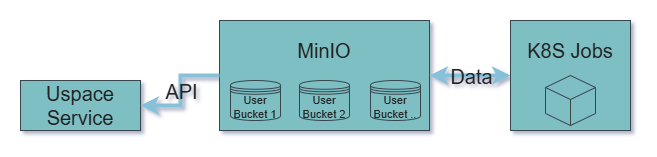
\includegraphics[width=1\textwidth]{Images/minio-overview.png}
  \caption{Minio Service Overview}
  \label{fig:minio-overview}
\end{figure}


MinIO is deployed as a Kubernetes StatefulSet backed by persistent volumes. This ensures durability of user data across pod restarts and facilitates scale-out configurations when needed.

Each service that interacts with MinIO is granted scoped credentials based on service identity. Access control is further enforced using path prefixes aligned with Fslite’s logical resource mappings. The system may optionally use signed URLs for temporary external access to datasets.



\section{Frontend and WebSocket Server}
\label{sec:frontend-wss}

\subsection{Overview}

The Frontend service acts as the primary user interface of the system, offering a web-based environment where users can register, log in, upload datasets, browse their resources, and submit batch analytical jobs. It is implemented using standard web technologies and communicates with backend services via RESTful APIs.

Beyond serving static HTML templates and handling client-side rendering, the Frontend plays a critical role in request mediation. It intercepts client requests, performs sanitization and validation, and attaches authentication tokens or service secrets where necessary. This enables secure and orchestrated communication between the user interface and core backend services, especially the Uspace API.

\subsection{WebSocket Server (WSS)}

The WebSocket Server (WSS) is implemented as a separate microservice that provides real-time, bidirectional communication capabilities between clients and the system. Its primary purpose is to support streaming logs, job status updates, and other event-driven feedback mechanisms related to job execution.

Clients interact with the WSS by issuing HTTP upgrade requests on a dedicated registration endpoint, specifying a Job ID (JID) and their desired role: \textit{Producer}, \textit{Consumer}, or \textit{JackOfAllTrades}. The server internally manages job-specific WebSocket channels. If a connection for the specified JID does not exist, it is initialized; otherwise, the client is added to the existing communication stream.

\begin{table}[H]
\centering
\begin{tabular}{|l|p{10cm}|}
\hline
\textbf{Role} & \textbf{Description} \\
\hline
\texttt{Producer} & Sends messages to the WebSocket channel. Typically used by job execution pods to stream logs, status updates, or results. \\
\texttt{Consumer} & Subscribes to a WebSocket channel and receives messages sent by the associated producer. Ideal for real-time job monitoring. \\
\texttt{JackOfAllTrades} & Can both send and receive messages within the WebSocket channel. Useful for debugging or hybrid clients. \\
\hline
\end{tabular}
\caption{Supported WebSocket communication roles}
\label{tab:wss-roles}
\end{table}


Additionally, an administrative endpoint allows forced disconnection of specific channels or participants, enabling control over job-specific streams.

\begin{figure}[h!]
  \centering
  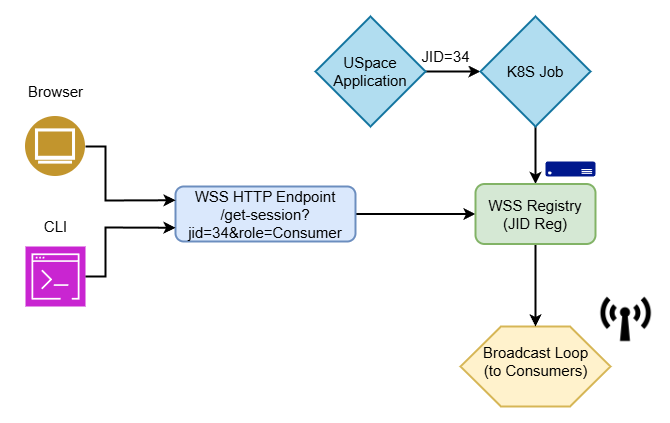
\includegraphics[width=1\textwidth]{Images/wss-blockdriagram.png}
  \caption{Wss Block Diagram}
  \label{fig:wss-blockdiagram}
\end{figure}

\subsection{Frontend–WSS Separation of Concerns}

While both the Frontend and WSS are part of the user-facing layer, they are deployed as independent services with different responsibilities. The Frontend focuses on rendering the user experience and forwarding REST-based job and resource operations to Uspace, while the WSS focuses on real-time feedback for asynchronous job execution.

This separation allows the system to maintain a clear modular boundary between interactive request-response behavior and event-driven streaming, simplifying system maintenance and scaling.


\subsection{Frontend Technology Stack}

The Frontend service is designed to offer a minimal yet responsive user experience, relying on standard web technologies and a server-side rendering model.

\begin{figure}[h!]
  \centering
  \begin{subfigure}[b]{0.15\textwidth}
    
\includegraphics[width=\textwidth]{Images/html.png}
    \label{fig:html5}
  \end{subfigure}
  \hfill
  \begin{subfigure}[b]{0.2\textwidth}
    
\includegraphics[width=\textwidth]{Images/Htmx_Logo.png}
    \label{fig:htmx}
  \end{subfigure}
  \hfill
  \begin{subfigure}[b]{0.1\textwidth}
    
\includegraphics[width=\textwidth]{Images/CSS3_logo_and_wordmark.svg.png}
    \label{fig:css}
  \end{subfigure}

  \begin{subfigure}[b]{0.25\textwidth}
    
\includegraphics[width=\textwidth]{Images/JavaScript-Logo.png}
    \label{fig:javascript}
  \end{subfigure}
  \hfill
  \begin{subfigure}[b]{0.2\textwidth}
    
\includegraphics[width=\textwidth]{Images/Go-Logo_Blue.png}
    \label{fig:golang}
  \end{subfigure}
  \hfill
  \begin{subfigure}[b]{0.15\textwidth}
    
\includegraphics[width=\textwidth]{Images/goGin_Logo.png}
    \label{fig:gogin}
  \end{subfigure}

  \caption{FrontEnd Technologies}
  \label{fig:authservices}
\end{figure}



\begin{itemize}
    \item \textbf{HTMX}~\cite{htmx-docs} is used as the main HTTP client, enabling dynamic content updates by issuing declarative AJAX requests embedded in HTML attributes. This reduces the need for complex JavaScript frameworks.
    
    \item \textbf{Go Templates} render HTML pages server-side using Go’s \texttt{html/template} engine. This allows safe and dynamic construction of views tied directly to backend logic.
    
    \item \textbf{Vanilla JavaScript} is used for basic DOM manipulation, file previews, and UI behaviors. The system avoids heavy client-side frameworks to maintain performance and reduce complexity.
    
    \item \textbf{CSS} is used to apply styling and layout. The design aims for clarity and usability, with lightweight responsive behavior for handling multiple screen sizes.
    
    \item \textbf{Gin Framework} in Go powers the backend of the Frontend service, handling routing, middleware, and template rendering.
\end{itemize}

Security is enforced via JWT-based middleware and service-to-service secret headers. All critical interactions (e.g., job submissions, resource uploads) are protected with authentication and validated on the server.

\begin{figure}[h!]
  \centering
  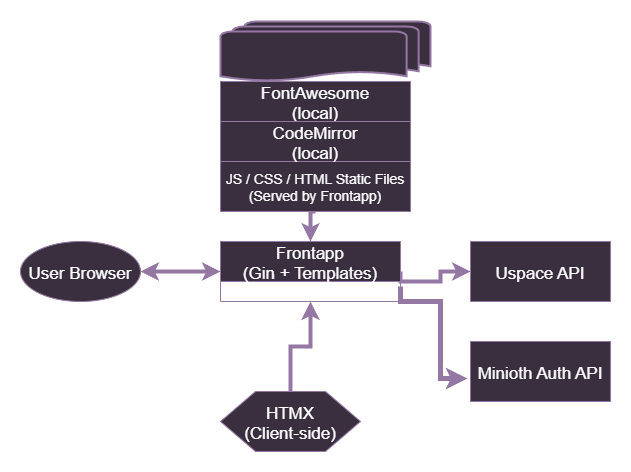
\includegraphics[width=1\textwidth]{Images/frontapp-blockdiagram.png}
  \caption{Frontapp Overview diagram}
  \label{fig:frontapp-overview}
\end{figure}

To support syntax-highlighted editing for user-submitted scripts (e.g., SQL, Python), the frontend integrates CodeMirror, a versatile in-browser code editor~\cite{codemirror}.

Interface icons, tool indicators, and status badges are rendered using the Font Awesome Free icon library~\cite{fontawesome}, providing visual consistency and accessibility.
Both technology stacks are served from Frontapp, bypassing any cdn.

\subsection{Integration}
Both the Frontapp and the Wss are integrated in the system as Kubernetes Deployments remaining stateless. There is also ephimeral logging, 
which can be used in the future.



\section{Kubernetes Integration}

Kubernetes functions as the orchestration backbone of the system. It is responsible for deploying, scheduling, and executing containerized jobs 
submitted by users. Uspace leverages Kubernetes Jobs to launch sandboxed environments in which user-specified tools (e.g., DuckDB, Octave) are 
executed. It also deployes each Microservice itself, tightening overall security and exposes only the desired service to the end user. In 
this case everything should be used and accessed via Frontapp.

Additionally, Kubernetes' Persistent Volume Claims (PVCs) or object storage access is used in allignment with StatefulSets to persist data. 
Everything deployed on K8S is namespaced. 

Each service is included with a Kubernetes Service and configured accordingly so that there is inter-service communication. There is also use 
for Node-Port Services for the system entrypoints.

Overall, the integration with Kubernetes allows the system to inherit properties such as fault tolerance, scaling, and container lifecycle management. 
It enables infrastructure-level abstraction so that users do not need to interact directly with Kubernetes primitives.
% Todo
